\chapter{Introduction}
\label{chp:Intro}

%%%%%%%%%%%%%%%%%%%%%%%%%%%%%%%%%%%%%%%%%%%%%%%%%%%%%%%%%%%%%%%%%%%%%%%

%Add in a story regarding the change from colocalization to thresholding
\section{Background}\label{sec:background}
\subsection{Motivation for mitophagy research}
The human body is a multicellular organism comprised of many different organs and tissues, each of which is composed of an immense number of different types of specialised cells working together to enable the biological functions that allow us to live and act. The vast majority of these cells contain a number of specialised components fulfilling a number of functions and important among them is the mitochondria. The mitochondrion is an organelle that has developed to efficiently process food molecules, absorbed by the body, and convert them into a form of chemical energy that is easily used by the other organelles within the cell. This is crucial as cells with specialised functions in turn have specialised organelles to achieve them and typically the energy requirement is relatively high. Due to chemical wear and tear from performing their functions, or due to external forces, the efficiency and health of mitochondria can diminish and at their worst can become a hindrance to the healthy supply of energy for the cell.\par When this occurs a process called mitophagy activates where the irreparably damaged mitochondria are flagged, isolated, and broken down for the biomolecules composing it to be reused by the cell~\cite{cell_phys_book}. There are two organelles involved in this process and they are the autophagosome, involved with isolating and transporting the flagged mitochondria, and the lysosome, triggering the decomposition process which breaks down the mitochondria. There is a risk though of this mitophagy not activating correctly, or being dysfunctional, and is associated with a number of human illnesses particularly those that are neurodegenerative such as Alzheimer's disease and Parkinson's disease~\cite{mito_diseases}. It is for this reason that research into the mechanisms behind mitophagy, the causes of the dysfunction, and the correction of it is of value.

\subsection{The investigation of mitophagy}
The investigation behind the causes of dysfunction in mitophagy, and methods by which to correct it, can be approached in a number of ways. For studying the regulation and correction of mitophagy dysfunction it is more accessible to observe the behaviours of the mitophagy-relevant organelles using cell cultures. These observations can be performed either visually, chemically, or both to determine which organelle behaviours are associated with functional or dysfunctional mitophagy. To achieve this, a common approach is to apply treatments that target specific factors (chemical, thermal, physical, etc.) that stress the mitochondria. Once the mitochondria are sufficiently stressed, mitophagy will be triggered allowing us to observe the actions of the mitochondria and involved organelles (autophagosomes and lysosomes). Treatments can target different factors to measure their influence in triggering mitophagy or can induce dysfunction in mitophagy. Visual observation of these events provides greater spatial information with regard to the organelles (position, size, count) especially with many interactions being spatial (engulfment, joining, separation, etc.) and is achieved through microscopy imaging.

\subsection{Preparation of images prior to analysis}\label{sec:intro_noise}
The purpose of imaging is to capture a representation of the specimen that can be measured by visual and image analysis with the former being performed by humans with qualitative (e.g. estimating the shape of the subjects in the image) or quantitative (e.g. manually counting each individual subject) measures while the latter is performed by machines through algorithms that are able to provide more detailed quantitative measurements (e.g. the calculated distribution of subject sizes within a population which provides measures such as the mean or variance of the sizes). An obstacle to the accuracy of both the visual and image analysis is image degradation which is the loss of image quality due to the presence of a number of factors in the image. There are a number of different factors causing this image degradation but the three most prominent are noise, distortion and artefacts. Noise typically causes a misrepresentation of the intensities within an image and generally acts as an additive component~\cite{digitize_noise_chapt}. Distortion is a deformation in the spatial representation of the specimen being imaged with the shape and position of structures primarily being affected. Artefacts are a broad group that refers to any anomalous elements in the image that do not fall under the prior factors and could affect the intensity or spatial representations of the specimen. A common attribute among these is that they are undesired in the image and either obscure the structures of interest, misrepresent their features (e.g. size, shape, texture, etc.); or describe non-existent, or unintended, structures. If this image degradation remains then analysis of the image is less reliable with the results being skewed depending on the degradation factors present. Unfortunately, there is always some degradation present in all images but the impact depends on both the quantity of these factors and the sensitivity of the features that are being analyzed (e.g. structures or structural features that are small or fine in size are usually more sensitive).\paragraph{Restoring image quality:} The restoration of image quality and clarity has motivated the development of a number of techniques over many years. These techniques typically aim to reduce the impact of the aforementioned factors such that the image becomes a closer representation of the specimen improving the accuracy and reliability of further analyses. These techniques have typically been developed to target specific factor(s) (e.g. removing specific types of noise or distortion specifically) with each having optimal conditions (e.g. consistent illumination, high contrast between foreground and background, etc.) to perform effectively and when these conditions are not met the outcomes can be unsatisfactory for any analysis. It is for this reason that the applied techniques need to be correctly chosen based on the factors present within the image. These techniques can be roughly grouped together based on their intended outcome whether it be deconvolution techniques reducing the distortion caused by microscope diffraction; denoising techniques which reduce the presence of noise; image enhancement techniques which emphasise or correct image properties such as improving contrast or smoothing unequal illumination across the image; and binarizing techniques which segment structures between the foreground and background with the foreground typically being what is of interest to analysis. These are merely categories and based on the criteria and desired granularity sub-groups can be made such as ``wavelet filters'' and ``patch-based filters'' which may still share overlapping outcomes. 
\paragraph{Binarizing techniques:} 
These techniques focus on the separation of pixels between a foreground and background resulting in a binary image. The application of this can be quite broad but for the purposes of this research, the binary separation of pixels allows clear differentiation between what is and is not of interest to succeeding analyses. A commonly employed set of techniques in image analysis, to achieve binarization, are thresholding techniques where numeric threshold(s) are calculated from the image and used to determine whether a pixel belongs to the foreground or background based on whether the pixel intensity is greater than the threshold or not, respectively~\cite{segmentation_book}.
Effective binarization enables the selectivity of structures that can be of particularly great benefit to any image analyses employing quantitative measurements that are highly sensitive to the image quality (e.g. Gaussian noise can greatly compromise structure count measurements). Through this, the measurements taken can be isolated to only the foreground structures where the degradation factors may be weaker.
\paragraph{Thresholding groups:}
As mentioned previously, thresholding is a common method of \\achieving binarization but typically falls into two groups for image processing. These are global thresholding and local thresholding methods with each having their own respective pros and cons.
\begin{multicols}{2}
\textbf{Global methods}
\begin{itemize}
    \item Relies on the image histogram to determine the threshold value.
    \item Applies this threshold to all image pixels naively.
    \item Sensitive to both distortions of the image histogram and localised variations in image intensity.
    \item Require few, if any, parameters for optimal performance.
\end{itemize}
\columnbreak
\textbf{Local methods}
\begin{itemize}
    \item Determines the threshold of each pixel by evaluating the intensity characteristics of the localised region centred on it.
    \item Robust to localised characteristics in images (e.g. variations in contrast around structures).
    \item Performance is dependent on one or more parameters that may need to be tuned for each image for optimal results.
\end{itemize}
\end{multicols}
Despite this, both methods can still be sensitive to other degradation factors present in the image regardless of whether a global or local method is used.

\subsection{High-throughput pre-processing}
High-throughput pre-processing is where the pre-processing of images is optimised for both speed and the resultant image quality. This is usually applied to large batches of images and can form part of a larger high-throughput analysis sequence with the goal of expediting image analysis while maintaining accuracy. To optimize the improvements to the image quality achieved by the pre-processing it is not uncommon to sequentially apply pre-processing techniques to images in a pipeline. This acts as a synergistic process where the outcomes of preceding techniques in the pipeline can optimize the conditions for succeeding techniques allowing them to produce higher quality outcomes than if they were applied in isolation. A key component of high-throughput analysis is speed which is achieved by minimizing interruptions in the pre-processing by using automated techniques that do not require parameters to be tuned to achieve adequate results. 


\section{Problem Statement}\label{sec:problem_state}
After imaging a large number of various cells, all under identical imaging conditions (e.g. resolution, brightness, gain, etc.), it is often the case that high-throughput pre-processing be implemented as part of preparing them for analysis.  This approach ideally enables efficient and effective pre-processing, thereby saving time for studies and projects dealing with extensive batches of images. However, the involvement of binarization in this process can pose a challenge to the goals of high-throughput pre-processing. \par Binarization is challenging in high-throughput pre-processing due to the constraints that automatic global and local thresholding methods can impose. Global thresholding has a high sensitivity to intensity-related factors (e.g. noise) and image properties, such as contrast or brightness, that affect the histogram particularly when these vary over localised regions of the image. This can result in inconsistent results that can vary greatly based on each image. Local thresholding is more robust to localised variations across the image and is unaffected by the histogram but the quality of the results is dependent on the parameter tuning. Parameter tuning is a human-involved process of adjusting parameter values to attain the most accurate thresholding results but can be time-consuming to perform and the degree of tuning necessary can be worsened by the presence of degradation factors. This results in a situation where global thresholds provide simplicity of application but uncertainty in behaviour while local thresholding can provide robust results given that the parameters are sufficiently tuned for each image, disrupting the pacing of the high-throughput pre-processing.\par This is not a constant where pre-selected parameter values may be sufficient for a local threshold technique or the intensity-related image properties are consistent enough that there is minimal variation for global thresholding techniques. Resolving this problem through a solution that provides both the robustness of local thresholds with the simplicity of global thresholds would provide more opportunities for studies requiring the pre-processing of large image batches to expedite this research and save time. Providing an effective binarization solution could reduce the outcome of poor binarization which ranges from the inclusion of noise as structures of interest for analysis or the exclusion of structures important to the study. While machine learning solutions to similar problems exist~\cite{machine_segment}, their performance can be dependent on both the type and quantity of data they are trained on but this training data can be expensive or time-consuming to acquire.

\section{Project objectives}\label{sec:objectives}
To resolve this problem of binarization in high-throughput pre-processing a system will be designed based on these objectives:
\begin{enumerate}
    \item Optimize the binarization outcomes without parameter tuning being required.
    \item Be an automated method that can be integrated into a high-throughput pipeline.
    \item Most provide results similar to or exceeding established methods such as global or thresholding methods in a high-throughput context (no parameter tuning).
\end{enumerate}
These objectives will guide the design of a deterministic binarization system which will be referred to as Improved Automatic Threshold (IAT).

\section{Scope}
The constraints on the expectations for the development and evaluation of this binarization solution are:
\begin{enumerate}
    \item Commonly extracted structure features of the image that can be quantified by existing libraries (e.g. scikit-image~\cite{scikit-image}, SciPy~\cite{scipy}, etc.)  will be used to determine the binarization. Structure count, structure volumes, intensity distribution across structures, and structure-specific intensities. Combinations and transformations (e.g. averages, derivatives, etc.) of these features will also be considered.
    \item The system will be agnostic to image resolution and freely be able to process 2D and 3D images.
    \item The developed method will be evaluated against existing automatic global and local thresholding methods both quantitatively, using metrics such as signal-to-noise ratio (SNR), and qualitatively. The qualitative evaluations will entail visual analysis of the thresholding outcomes and will also be compared to manually thresholded images but not as extensively as the quantitative evaluation due to time constraints.
    \item This research is pursued application to imaging relevant to the study of mitophagy thus only the imaged mitochondria, autophagosomes, and lysosomes will be used for development and evaluation.
    \item Only images for a single type of microscopy will be used for both the development and evaluation of this method due to both time and resource constraints.
\end{enumerate}

%The Memantine research investigated the impact of Memantine, a medication, on the mitophagy process with a particular focus on the relationship between its influence on mitophagy relative to the concentration of the medication. There were multiple data sets collected that were acquired through fluorescence microscopy imaging to provide further data for both supporting more reliable conclusions from the data and to compensate for challenges in the data collection. It was found that there were challenges in the data collection were images with too much noise, weak fluorescence signals from objects of interest and non-specific fluorescent probes (staining more than the intended objects e.g. a mitochondria stain also staining the cytosol of the cell) increased the difficulty of forming accurate analysis and observations of those samples thus more was required. 


\section{Contributions}
Contributions made through this research were to the paper \textit{The Highs and Lows of Memantine—An Autophagy and Mitophagy Inducing Agent That Protects Mitochondria}~\cite{sholto_research} by assisting in sample pre-processing and image quality evaluation prior to analysis. Further contributions that are discussed are the potential contributions that this research could provide towards the image analysis, and related, fields.
\subsection{Contributions towards the Memantine research paper}
The IAT developed in this project originated from the application in high-throughput pre-processing of mitophagy-related organelle images to expedite data set preparation for mitophagy analysis. Coincidentally, research regarding the application of Memantine treatments and the analysis of its effects on mitophagy behaviour~\cite{sholto_research} was pursued. Despite the IAT project shifting focus from mitophagy analysis to image pre-processing, with a focus on mitophagy-related organelle images, support was provided to the Memantine research with regard to the image pre-processing and the evaluation of the image quality prior to mitophagy analysis. 

\paragraph{First contribution:} 
The development of a pre-processing pipeline macro for FiJi~\cite{Fiji_paper} to automate the pre-processing of 3D confocal fluorescence microscopy images of cellular organelles which are mitochondria, lysosomes, and autophagosomes. The pipeline used was based off of the pipeline described in \cite{PipelineDecon-Chaudhry} (excluding the binarization and all succeeding algorithms) with adjustments made detailed in Section \ref{sec:preprocess_applied}.

\paragraph{Second contribution:} 
With pre-processing having been applied, the quality of these images were evaluated under three criteria:
\begin{enumerate}
	\item Sufficient contrast of the structures of interest against the background, and any residual noise, for accurate differentiation.
	\item The lack of fluorescence falsely describing in-focus structures originating from either out-of-focus fluorophores, fluorescence cross-talk, and autofluorescence.
	\item Confident clustering of organelles in the images between separate cells if present.
\end{enumerate}
The first criterion being met implies that structures of interest can be differentiated and selected for algorithmic analyses where those results could be disturbed by erroneously including noise. The second criterion being met implies that aberrations in the image that are more challenging to automatically remove, without degrading the image signal, are not strongly present and will not distort measured results. The final criterion being met implies that per cell measurements are possible to capture for an image which is necessary for certain analyses.

\subsection{Contributions towards relevant fields}
The fields of relevance to this research are image analysis, with the focus on image binarization, and cellular physiology, as the data used in throughout the IAT development involved cellular organelle images. This will provide a binarization solution accessible to those with low expertise in image pre-processing while providing viable results particularly for high-throughput applications. For image analysis, the contribution will be the establishment of a new automated thresholding method with a novel approach to approximating binarized images. 

\section{Structure of thesis}
This thesis is composed of 6, including Chapter 1, with the remaining 5 Chapters summarised below:\par
\textbf{Chapter \ref{chp:Background}} provides context around many facets of this research project to build a fundamental understanding of certain decisions in the system design and the phenomena that are observed. These fundamentals are composed of context for the organelles being imaged in regard to their characteristics; the microscopy techniques used and how they function; a high-level overview of the pre-processing method groups and the roles each play in improving image quality; and specific methods that are of note to the system design.\par
\textbf{Chapter \ref{ch:methodology}} will present the rationale behind the preparation of the specimen which is imaged, the pre-processing techniques applied to improve the image quality, and the design of the system IAT to binarize the objects of interest with observations and tests to justify said design choices.\par
\textbf{Chapter \ref{ch:results}} will present and discuss the performance results of the IAT against established thresholding methods.\par
\textbf{Chapter \ref{ch:conclude}} will provide a conclusion regarding the performance of the IAT method, the shortcomings, and improvements to be made through future work.  

\begin{figure}[h!]
    \centering
    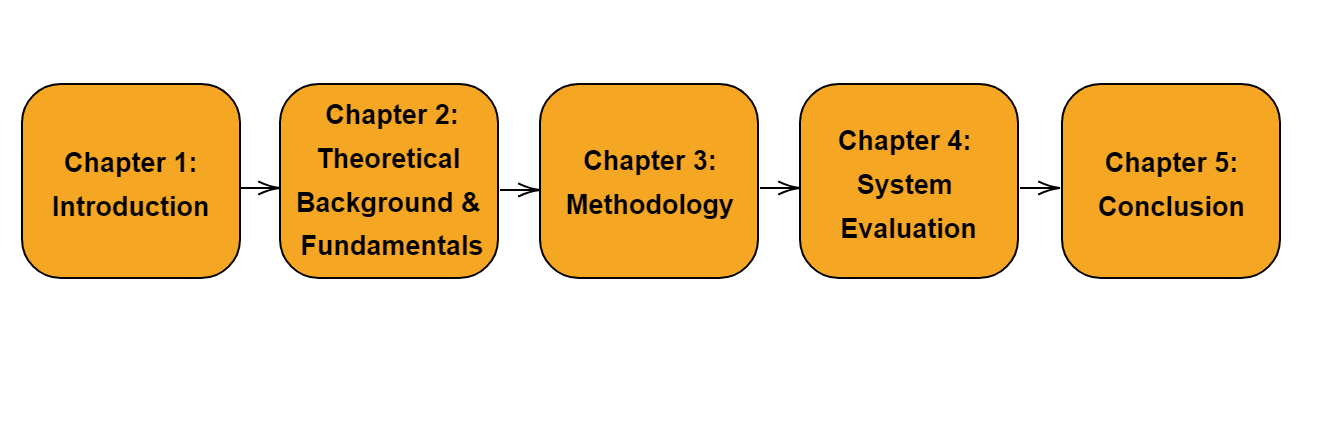
\includegraphics[width=\linewidth]{figs/thesis_structure_diagram.png}
    \caption{Diagram of thesis structure}
    \label{fig:thesis_struct_diag}
\end{figure}
 